\documentclass[12pt]{report}
\usepackage[margin=1in]{geometry}
\usepackage{hyperref}
\usepackage{graphicx}
\usepackage{amsmath}
\usepackage{enumitem}
\usepackage{float}

\title{Week 3 Report}
\author{Dhanush Balusa}
\date{June 4, 2025}

\begin{document}

\maketitle

\chapter*{Research}

\textbf{Coordinate System: True Equator, Mean Equinox (TEME)}
\begin{itemize}
  \item True Equator: The coordinate plane uses the actual orientation of Earth’s equator at a given time.
  \item Mean Equinox: The reference for the vernal equinox does not include short-period variations like nutation (periodic "wobbling" motion of Earth's rotation axis caused by the gravitational influence of the Moon and Sun on Earth's equatorial bulge).
  \item \url{https://astronomy.stackexchange.com/questions/44140/can-someone-explain-to-me-the-teme-reference-frame-in-defining-orbital-coordinat}
\end{itemize}

\textbf{SGP4}
\begin{itemize}
  \item Note: Last week I learned that TLEs are not accurate for long periods of time and that they are updated frequently.
  \item \url{https://conference.sdo.esoc.esa.int/proceedings/sdc6/paper/41/SDC6-paper41.pdf}
\end{itemize}

\textbf{Other resources:}
\begin{itemize}
  \item \url{https://naif.jpl.nasa.gov/pub/naif/toolkit_docs/Tutorials/pdf/individual_docs/17_frames_and_coordinate_systems.pdf}
\end{itemize}

\chapter*{Previous Code}
My code from the previous week calculated the approach conditions between the ISS and NOAA 15.
\begin{figure}[H]
    \centering
    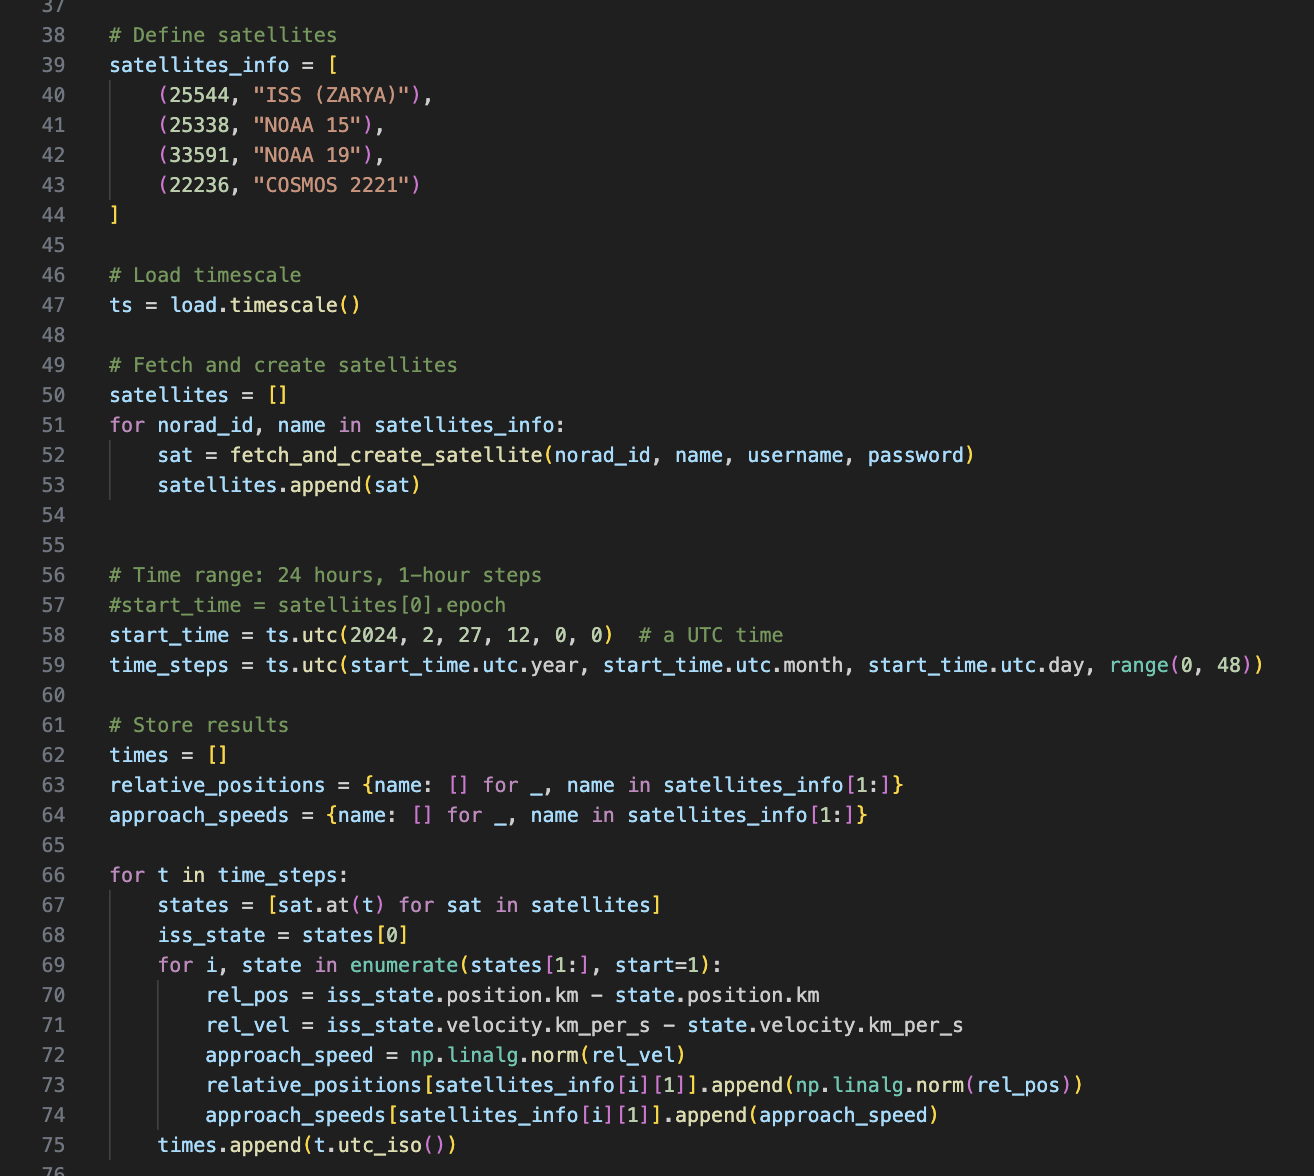
\includegraphics[width=0.8\textwidth]{figure_week_2_code.png}
    \caption{Code from week 2 calculating the approach conditions between ISS and a couple of other satellites}
    \label{fig:code}
\end{figure}

\chapter*{Code Changes}

Based on the feedback from last week’s team meeting, I decided to make the following changes:

\begin{enumerate}
  \item \textbf{My first change was to check if the TLE data is fetched correctly.}

  \textit{Observation:} All the TLE data is fetched correctly, it is the most recent TLE data (as of 5/28/2025).
  
  \begin{figure}[H]
    \centering
    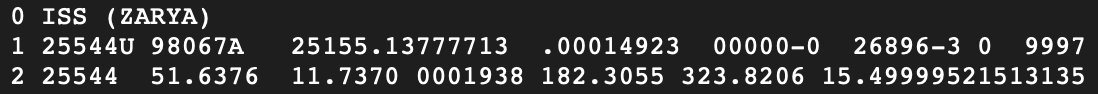
\includegraphics[width=0.8\textwidth]{figure_week_3_tle_space_track.png}
    \caption{TLE data from Space Track for ISS (ZARYA)}
    \label{fig:tle_space_track}
  \end{figure}

  \begin{figure}[H]
    \centering
    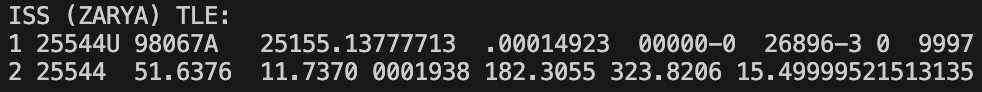
\includegraphics[width=0.8\textwidth]{figure_week_3_tle_fetched.png}
    \caption{TLE data fetched from Space Track's API for ISS (ZARYA)}
    \label{fig:tle_fetched}
  \end{figure}

  \item \textbf{My second change was to fetch historical TLE data.}

  \begin{figure}[H]
    \centering
    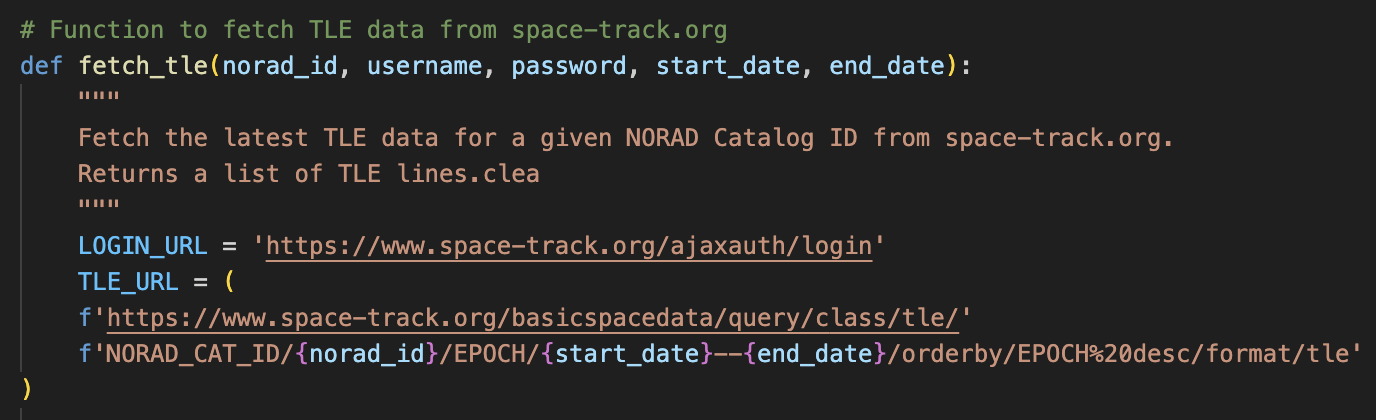
\includegraphics[width=0.8\textwidth]{figure_week_3_historicalTLE.png}
    \caption{I updated the fetch\_tle functiion to get historical TLE data}
    \label{fig:historical_tle}
  \end{figure}

  \textit{Observation:} It seems like the code fetches the TLE data correctly.\\

  \item \textbf{My third change was to compare the approach conditions of the TIMED satellite and Cosmos 2221.}
    
  \begin{figure}[H]
    \centering
    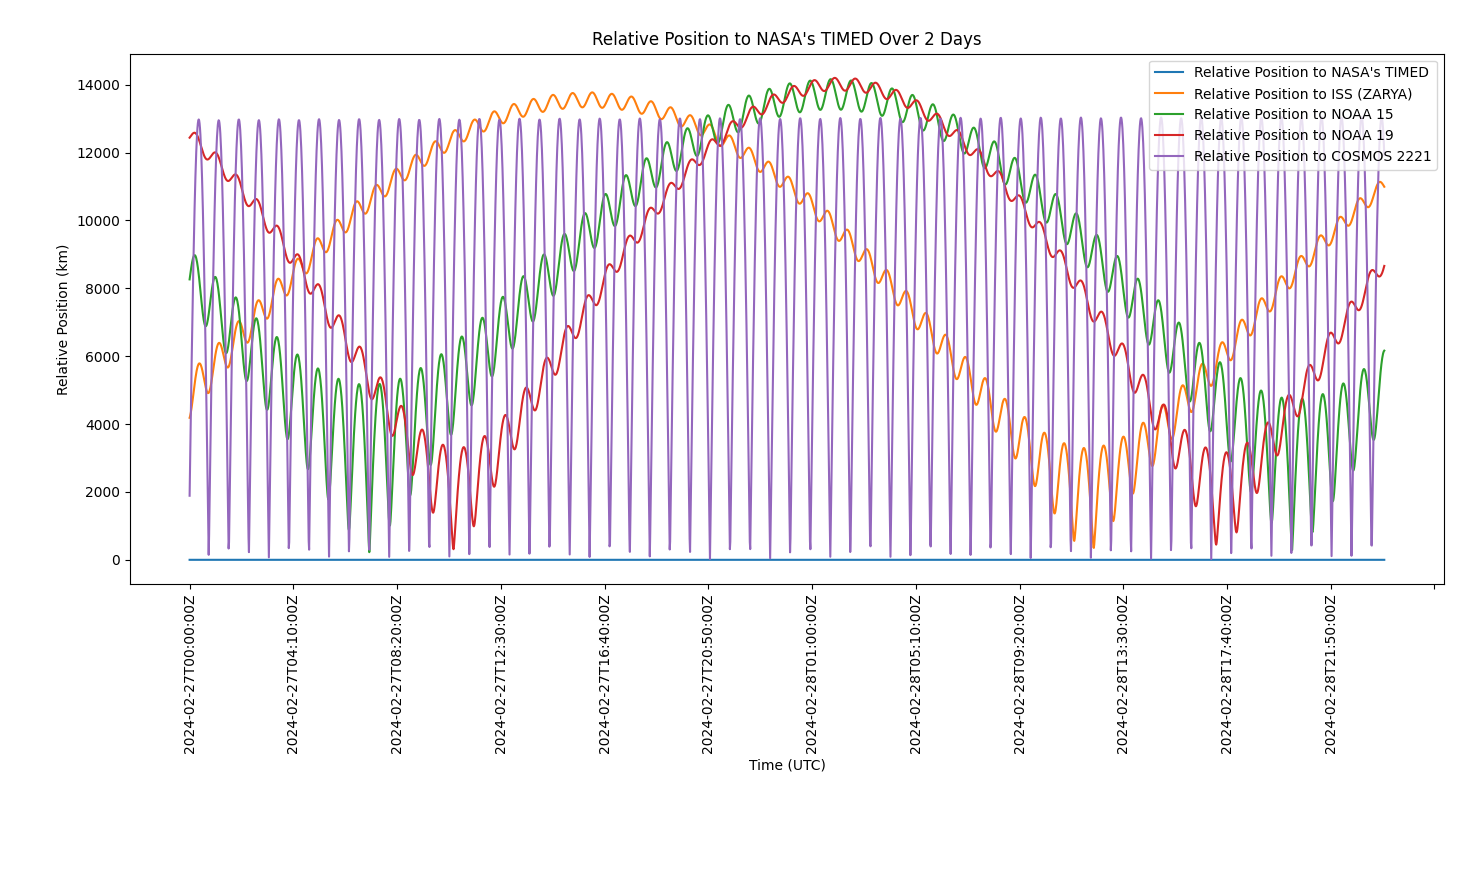
\includegraphics[width=0.8\textwidth]{figure_week_3_TIMEDvCos2221_plot.png}
    \caption{NASA's TIMED satellite's near miss with Cosmos 2221}
    \label{fig:timed_cosmos_plot}
  \end{figure}
  \textit{Note:} Cosmos 2221 is the odd satellite out, why? Why does it follow a sinusodal patern in so quickly? If I try using GMAT with TLEs that could help me.

    \begin{figure}[H]
      \centering
      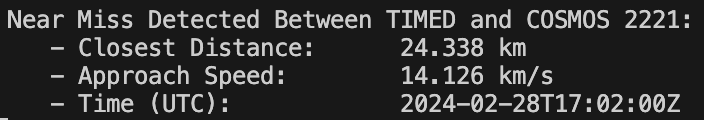
\includegraphics[width=0.8\textwidth]{figure_week_3_TIMEDvCos2221.png}
      \caption{Approach conditions of TIMED satellite and Cosmos 2221.\\}
      \label{fig:timed_cosmos_approach}
    \end{figure}
    \textit{Issue:} The correct time is around 6:30 UTC on February 28, 2024. The approach speed is fluctuating too much, I need to check the code for errors.\\


  \newpage
  \item \textbf{My fourth change was adding Iridium 33's collision with Cosmos 2251 from 2009.}
  
  \begin{figure}[H]
    \centering
    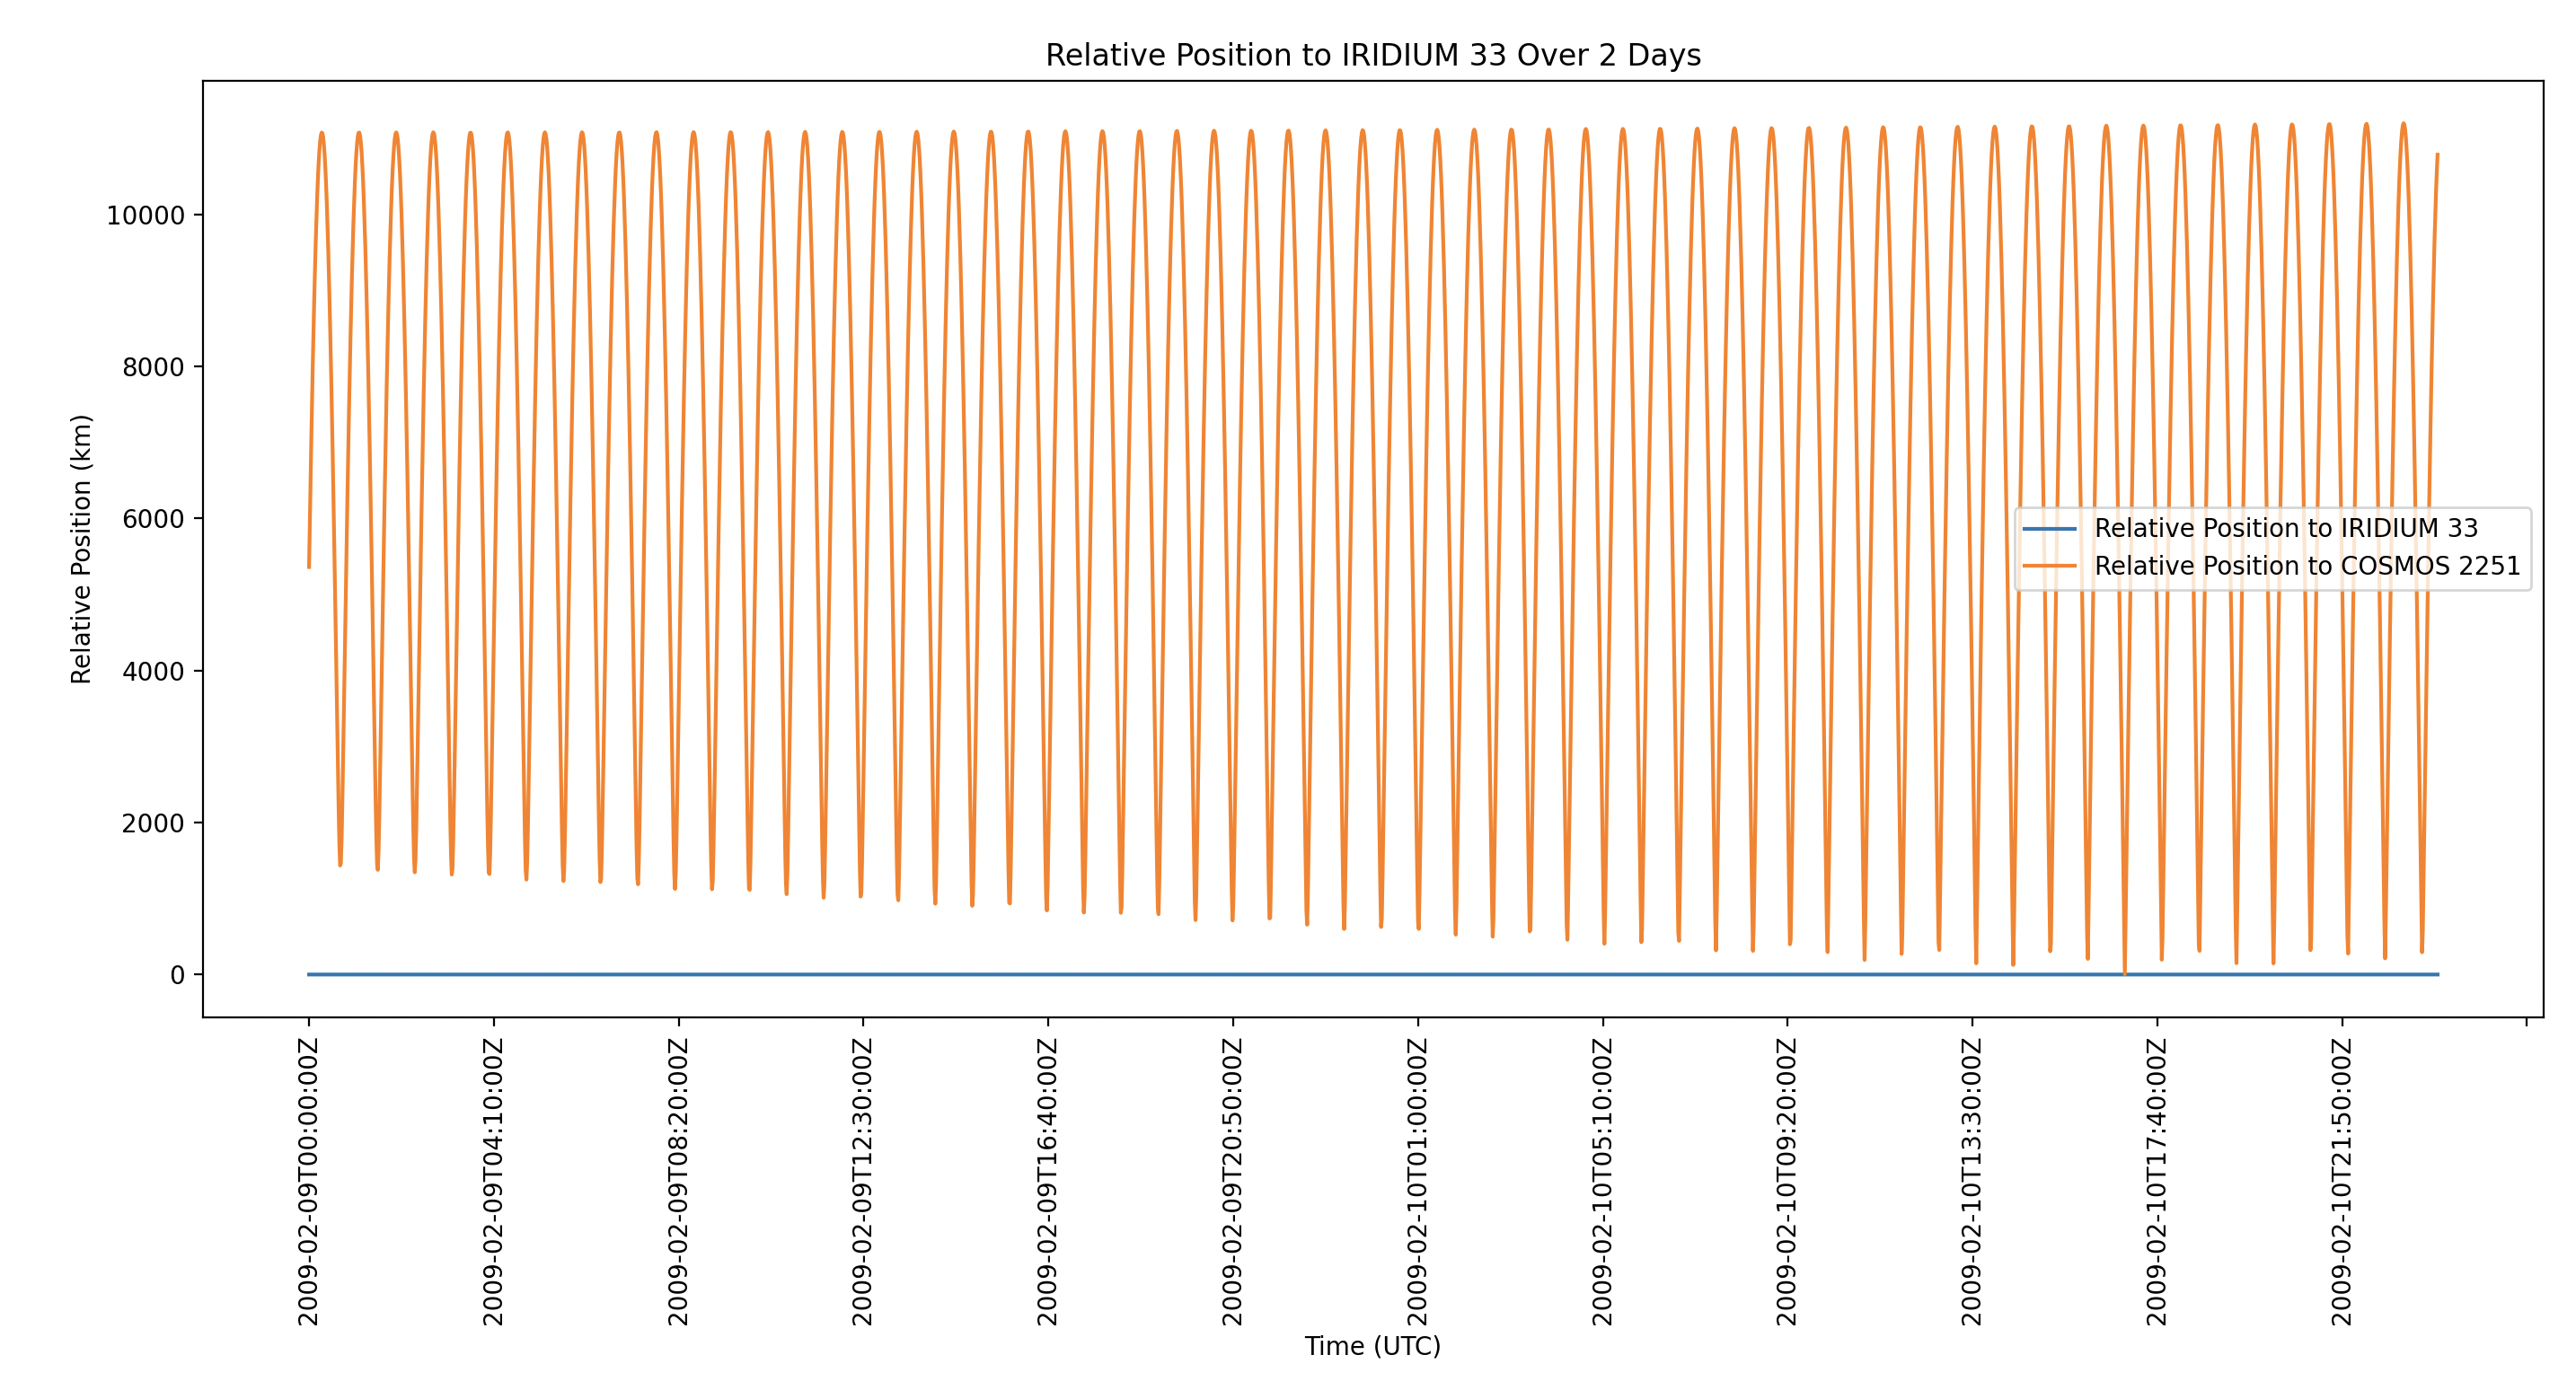
\includegraphics[width=0.8\textwidth]{figure_week_3_ird33vscos2251_plot.png}
    \caption{Iridium 33 collides with Cosmos 2251 around 16:56 UTC on February 10, 2009.}
    \label{fig:iridium_collision_plot}
  \end{figure}

  \begin{figure}[H]
    \centering
    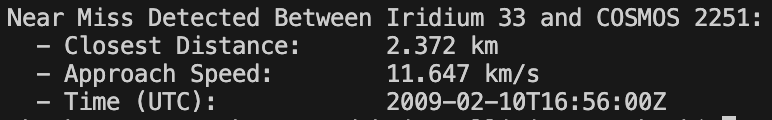
\includegraphics[width=0.8\textwidth]{figure_week_3_ird33vscos2251.png}
    \caption{Approach conditions of Iridium 33 collision with Cosmos 2251.}
    \label{fig:iridium_collision_approach}
  \end{figure}
  
    \textit{Observation:} The code accurately calculates the time of the collision.\\
    \textit{Next steps:} I need to calculate and cross check the approach speed and angle of the collision. Since this test case works I need to utilize it too test all my calculations. Also I need to simulate this collision using GMAT and see how accurate my calculations were.\\
    \textit{Issue:} Why can't I get the TIMED satellite and Cosmos 2221 to work?\\
    \textit{Note:} The time matches but the approach speed has to be checked.\\

  \url{2009 collision: https://en.wikipedia.org/wiki/2009_satellite_collision}

\end{enumerate}

\chapter*{Next Steps}
\begin{itemize}
  \item Read more about the error in SGP4.
  \item Research if the compact sinusoid patern is correct. I don't understand why the relative position is fluctuating so quickly.
  \item Calculate the angle of approach, cross check with GMAT. Check the approach speed too.
  \item Loop through all the TLEs in the file and calculate the approach conditions for each satellite if it is within a certain distance (e.g., 100 km) of the ISS.
  \item Make my code a usable function so Catherine can just call it. Input? \textrightarrow{} Output (angle and approach speed)
\end{itemize}

\end{document}